\documentclass{article}
\title{Getting Started with LLGL}
\author{Lukas Hermanns}
\date{\today}

\usepackage{listings}
\usepackage{color}
\usepackage{pxfonts}
\usepackage{geometry}
\usepackage[T1]{fontenc}
\usepackage{xspace}
\usepackage{hyperref}
\usepackage{graphicx}
\usepackage{float}

\geometry{
	a4paper,
	left=15mm,
	right=15mm,
	top=20mm,
	bottom=20mm
}

\begin{document}

\definecolor{brightBlueColor}{rgb}{0.5, 0.5, 1.0}
\definecolor{darkBlueColor}{rgb}{0.0, 0.0, 0.5}

\def\LLGL{\textcolor{darkBlueColor}{LLGL}\xspace}

\lstset{
	language = C++,
	basicstyle = \footnotesize\ttfamily,
	commentstyle = \itshape\color{brightBlueColor},
	keywordstyle = \bfseries\color{darkBlueColor},
	stringstyle = \color{red},
	frame = single,
	tabsize = 4,
	showstringspaces=false,
	numbers=none
}

\maketitle


%----------------------------------------------------------------------------------------
%	INTRRODUCTION
%----------------------------------------------------------------------------------------

\section*{Introduction}

\LLGL (Low Level Graphics Library) is a thin abstraction layer for graphics APIs such as
OpenGL, Direct3D, and Vulkan. The library is written entirely in C++11, so you'll
need a modern C++ compiler, i.e. at least \textbf{VisualC++ 2013} for Windows,
\textbf{g++ 4.8} for Linux, or \textbf{Clang 3.1} for MacOS.


%----------------------------------------------------------------------------------------
%	BUILD PROCESS
%----------------------------------------------------------------------------------------

\section*{Build Process}

\subsection*{Dependencies}

\subsubsection*{GaussianLib}

The only required dependency is the header-only library
\href{https://github.com/LukasBanana/GaussianLib}{\textsc{GaussianLib}},
which is used for basic linear algebra computations with vectors and matrices.

\subsubsection*{OpenGL}

To build the OpenGL render system you need the OpenGL extension header files and an up-to-date graphics driver.
For Windows the header files \texttt{glext.h} and \texttt{wglext.h} are required.
For Linux the header files \texttt{glext.h} and \texttt{glxext.h} are required.
For MacOS no header files need to be downloaded, since the OpenGL version depends on the OS version.
You can find the header files at the \href{https://www.opengl.org/registry/#headers}{OpenGL registry page}.
Place the header files in the \texttt{include/GL/} folder of your compiler environment
or add the include path later in your build settings.

\subsubsection*{Direct3D}

Since VisualStudio 2013 the DirectX framework (of which Direct3D is a part of) is included within
the VisualStudio setup, so no further SDK needs to be installed.

\subsubsection*{Vulkan}

To build the Vulkan render system you need the \href{https://lunarg.com/vulkan-sdk/}{Vulkan SDK},
and of course a graphics driver which supports at least Vulkan 1.0.

\subsection*{Build Tool}

To build the \LLGL project files you need the build tool \href{https://cmake.org/}{CMake 2.8} or later.
The build process is now demonstrated with the CMake GUI on Windows, but it can also be configured
on a command line (more about this see \href{https://cmake.org/runningcmake/}{cmake.org/runningcmake}).

Set the source directory (``Where is the source code:'') to the \LLGL repository
and set the build directory (``Where to build the binaries'') where you want your project files.
In this example (see \ref{fig:cmake_mask1}) the source directory is \texttt{<\dots>/LLGL/repository}
and the build directory is \texttt{<\dots>/LLGL/build\_msvc14} because the project files are build
for MSVC14 (VisualStudio 2015).

Now set the \textsc{GaussianLib} include directory (in this example \texttt{<...>/GaussianLib/repository/include})
and click on ``Configure''. If everything worked quite well, you should see the message ``Configuring done''
in the lower box. To finally create the project files, clock on ``Generate''.
Then your project files should be located in the build directory you just set up previously.

\begin{figure}[H]
	\centering
	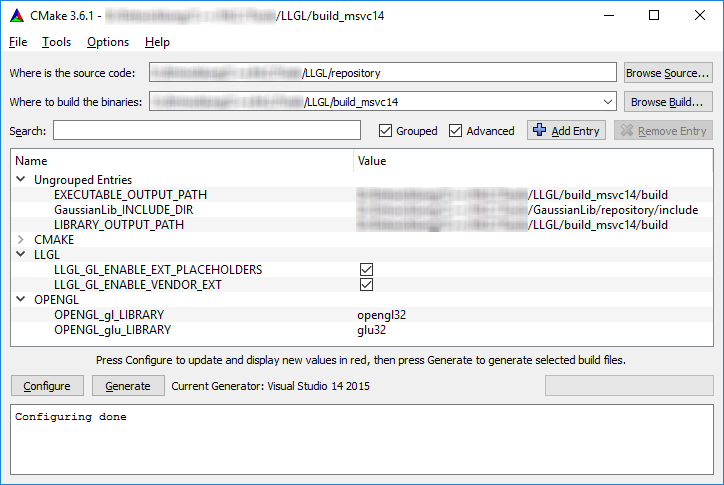
\includegraphics[width=0.9 \textwidth]{cmake_mask1}
	\caption{CMake GUI mask to set up the project files for VisualStudio 2015 (MSVC14).}
	\label{fig:cmake_mask1}
\end{figure}

There are a few options you can switch on and off, which will enable or disable the respective macro
when you compile the project:
\begin{itemize}
	\item \texttt{LLGL\_GL\_ENABLE\_EXT\_PLACEHOLDERS} \\
	Specifies whether OpenGL extensions should be replaced by placeholder procedures
	when they are not available. This may help debugging and should not influence the runtime performance.
	
	\item \texttt{LLGL\_GL\_ENABLE\_VENDOR\_EXT} \\
	Specifies whether vendor specific OpenGL extensions should be enabled or disabled.
	One of these extensions is for conservative rasterization
	(\texttt{GL\_NV\_conservative\_raster} and \texttt{GL\_INTEL\_conservative\_rasterization}) for instance.
	These extensions will only be loaded and used by the runtime if they are available on the host platform.
\end{itemize}


%----------------------------------------------------------------------------------------
%	API OVERVIEW
%----------------------------------------------------------------------------------------

%\newpage

%\section*{API Overview}

%LLGL has a very simple and unified API design.

%\begin{lstlisting}
%class RenderSystem
%{
%	static shared_ptr<RenderSystem> Load(string moduleName);
%}
%\end{lstlisting}


%----------------------------------------------------------------------------------------
%	HELLO TRIANGLE
%----------------------------------------------------------------------------------------

\newpage

\section*{Hello Triangle}

After we have set up and build the library, we can start rendering some geometry.
Our example will consist of a single C++ source file (e.g. ``\texttt{main.cpp}'') and two shader files
(e.g. ``\texttt{vertex.glsl}'' and ``\texttt{fragment.glsl}'').
The include path for a project, that uses \LLGL, must be set to \texttt{\textit{<your-LLGL-repository>}/include/},
and the \LLGL library file must be added to the linker (for Windows this is ``\texttt{LLGL.lib}''
when compiling in Release mode and ``\texttt{LLGLD.lib}'' when compiling in Debug mode).
All the other library files don't need to be added to the linker (e.g. ``\texttt{LLGL\_OpenGL.lib}''),
since the respective renderer module is loaded at runtime.

Now let's start with a small example. At first we need to include the header files.
The main header we need is \texttt{LLGL/LLGL.h} where the entire \LLGL interface is declared.
For our example we also need basic I/O classes from \texttt{iostream} for standard output and \texttt{fstream}
to read the shader files:
\begin{lstlisting}
#include <LLGL/LLGL.h>
#include <iostream>
#include <fstream>
\end{lstlisting}

Next we define the C++ main function and wrap the entire example code into a large \texttt{try-catch} block,
to quit the application with a meaningful error message if any failure happens:
\begin{lstlisting}
int main() {
    try {
        /* example code here ... */
    } catch (const std::exception& e) {
        std::cerr << e.what() << std::endl;
    }
    return 0;
}
\end{lstlisting}

To create an \LLGL renderer instance in our main function, we load a renderer module
(a \textit{module} here denotes a dynamic shared library)
from the static \texttt{Load} function of the \texttt{RenderSystem} interface:
\begin{lstlisting}
std::shared_ptr<LLGL::RenderSystem> renderer = LLGL::RenderSystem::Load("OpenGL");
\end{lstlisting}
Here we could actually use the C++11 keyword \texttt{auto} to simplify the code,
but for explanation purposes we keep the types explicit.
Most creation or load functions return a new instance wrapped in a \texttt{std::unique\_ptr},
but in this case \LLGL needs to keep track of the instance to check if it has already been expired,
which is only feasible with an \texttt{std::shared\_ptr}.

Moreover, most functions use enumerations instead of strings to specify some type, but in this case
a module can be loaded dynamically at runtime and further modules can be added or removed independently.
Therefore the renderer module is specified by a string (here ``OpenGL''). Other modules are
named ``Direct3D11'', ``Direct3D12'', and ``Vulkan''.
Whenver you load a new renderer, there must not remain any references to this shared object,
because only a single renderer can be loaded at a time.
When this shared object expires, all objects allocated by this renderer will be deleted automatically.

If loading the renderer failed, an \texttt{std::runtime\_error} exception will be thrown,
which can be cached to show an erorr message and/or load another renderer module instead.
This can be very handy if a specific Direct3D version is not installed on the host Windows platform,
so another Direct3D version or OpenGL renderer can be loaded as fallback
without disturbing the user with akward error messages and program crashes.

After we created the renderer we need a graphics context to draw into.
This is done by the \texttt{CreateRenderContext} function which takes a descriptor structure:
\begin{lstlisting}
LLGL::RenderContextDescriptor contextDesc;
{
    contextDesc.videoMode.resolution = { 800, 600 };
}
LLGL::RenderContext* context = renderer->CreateRenderContext(contextDesc);
\end{lstlisting}
This is a minimal example for the render context descriptor. There are much more attributes
to specify anti-aliasing, vertical-synchronisation, etc.
See the API documentation for more information about these attributes.

This render context will create its own window, but we could also specifiy our own one.
However, in this example we keep it simple. To access this window and change the title,
we use the \texttt{GetWindow} function of the \texttt{RenderContext} interface
which returns a constant reference to its window:
\begin{lstlisting}
context->GetWindow().SetTitle(L"Hello Triangle with LLGL");
\end{lstlisting}
Since some platforms (such as Win32) support Unicode window titles, our string literal starts with the `L' token.


%----------------------------------------------------------------------------------------
%	APPENDIX
%----------------------------------------------------------------------------------------

%\newpage

%\section*{Appendix}

%Foo bar ...






\end{document}
